\documentclass[letter,11pt]{article}

\usepackage[margin=1in]{geometry}

\usepackage{graphicx,url}
\usepackage{subfig}

\usepackage{amsmath}
\usepackage{amsfonts}
\usepackage{mathtools}
\usepackage{multicol}
\usepackage{blkarray}
\usepackage{dsfont}

\parskip=11pt

\title{Performance and Economic Models in the Cloud:\\
Case of Serverless Computing and Spot Instances}
\date{}

\begin{document}

\maketitle

\section{System}

There are two forms of computing available in the cloud: Spot Instance and Serverless Computing.

In \textbf{Spot Instances}, the client rents a Virtual Machine (VM), which has a fixed set of physical resources such as CPUs and cores, main memory, long term storage and bandwidth. The Virtual Machine (VM) can run multiple containers. Assume that VMs alternate between idle and busy. There is a startup delay for VM to run containers.
The client pays per second for the duration that the VM runs. The price of the VM fluctuates based on supply. The VM only executes as long as the price is below the client's specified price threshold.

In \textbf{Serverless Computing}, the cloud provider provisions containers and executes the client's functions. The cost is determined by the function's execution duration (every 100ms) and number of executions.  

\section{Key Questions}
\begin{itemize}
\item
To reduce the cost, which form of computing should be used?
\item
Does it make business case to use both forms of computing? If so, how much computing should be done by Serverless? How many VMs should be allocated?
\end{itemize}

\section{Performance Model}

To model \textbf{Serverless Computing}, assume function calls arrive according to a Poisson process with rate $\lambda_s$. Each function runs in the server for a random amount of time, exponentially distributed with rate $\mu_s$. 

To model \textbf{Spot Instances}, we start with a simpler case with only one VM and fixed price for the VM. Assume there is a setup time, exponentially distributed with rate $\gamma$. Assume the functions arrive according to a Poisson process with rate $\lambda_m$. Each function runs in the VM for a random amount of time, exponentially distributed with rate $\mu_m$. 

\begin{figure}[h]
    \centering
    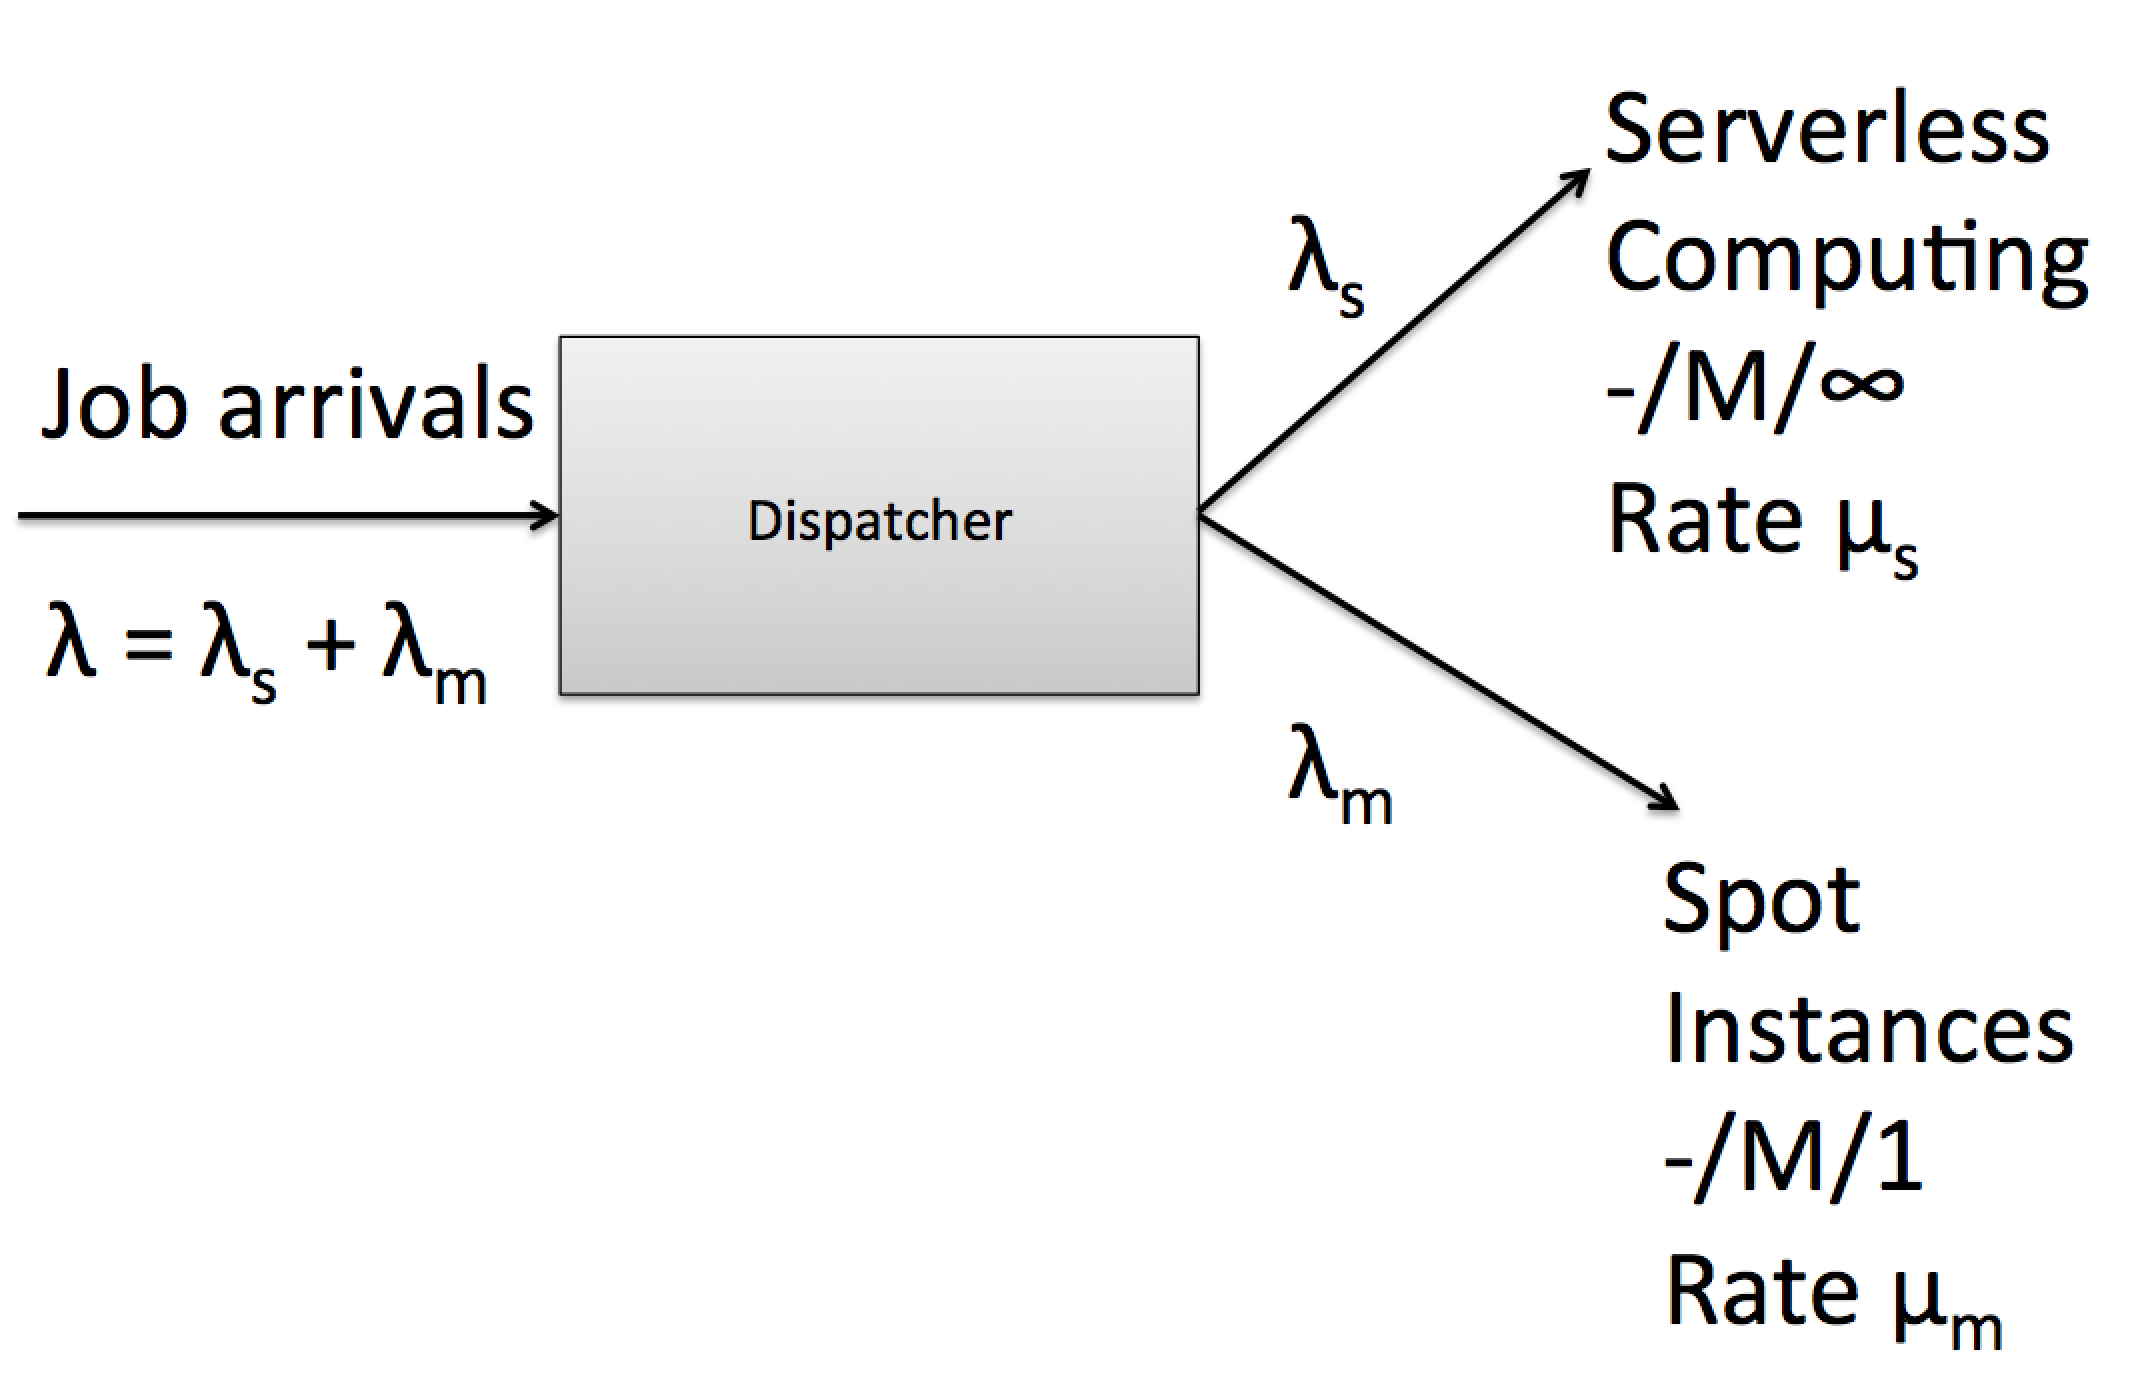
\includegraphics[width=0.5\textwidth]{dispatcher}
    \caption{Performance model for VMs and serverless computing in a cloud server.}
    \label{fig:model}
\end{figure}

\subsection{Cost Model} 

\textbf{Serverless} : $C_s(t) = \alpha_s t$ (for each job that takes time t) \\ \\
\textbf{Spot Instances}:  $C_m(t) = \alpha_m t$ (for each VM up for time t including setup time) 

\subsection{Cost Analysis}

In this section, we compute the expected cost per unit time for serverless and spot instances. 

\subsubsection{Serverless}

For serverless, the cost is dependent on the number of function executions $E[Q]$. \\
Expected cost per unit time = $\alpha_s E[Q]$ = $\frac{\alpha_s \lambda_s}{\mu_s}$

\subsubsection{Spot Instances} 

\begin{itemize}
\item \textit{Case 1: VM ON always} 

Expected cost per time = $\alpha_m$ 

\item \textit{Case 2: single VM ON only to serve jobs} 

In this case, the expected cost per unit time consists of cost to serve jobs as well as the cost for setting up the first instance.

Cost to serve jobs  = $\frac{\alpha_m \lambda_m}{\mu_m}$ \\ \\
Computing cost for first instance: \\
Time idle = $T - T \rho$ where T is the total time and $\rho$ is busy time of VM \\
Number of occurrences when first instance is used (a.k.a. number of times 	queue is empty) = $\frac{T - T \rho}{\frac{1}{\lambda_m}}$
= $\lambda_m (T - T \rho)$ = $\lambda_m T (1 - \rho)$ \\
Cost for first instance = $\alpha_m$ * number of times queue is empty * setup time cost = $\frac{\alpha_m \lambda_m (1 - \rho)}{\gamma} $ \\ \\
Expected cost per unit time = $\frac{\alpha_m \lambda_m}{\mu_m} + \frac{\alpha_m \lambda_m (1 - \rho)}{\gamma} $ 

Substituting $\rho$ with $ \frac{\lambda_m}{\mu_m}$,

Expected cost per unit time = $\frac{\alpha_m \lambda_m}{\mu_m} + \frac{\alpha_m \lambda_m (1 - \frac{\lambda_m}{\mu_m})}{\gamma} $ \\ \\
= $\frac{\alpha_m \lambda_m}{\mu_m} + \frac{\alpha_m \lambda_m (\mu_m - \lambda_m)}{\mu_m \gamma} $ \\ \\
= $\alpha_m \lambda_m(\frac{1}{\mu_m} + \frac{\mu_m - \lambda_m}{\mu_m \gamma}) $

\item \textit{Case 3: Multiple VMs ON only to serve jobs} 

This case increases the number of VMs that are utilized as opposed to a single VM in case 2. Assume that $i$ is the number of VMs, each of which can be turned ON and OFF. The arrival rate of jobs for each VM is equal, where the rate is $\frac{\lambda_m}{i}$.

Cost to serve jobs (same as in case 2)  = $\frac{\alpha_m \lambda_m}{\mu_m}$

Cost for first instance for multiple VMs = sum of cost for instance for each VM

From case 2, cost for first instance for a single VM for arrival rate $\lambda_m$= $\alpha_m \lambda_m(\frac{1}{\mu_m} + \frac{\mu_m - \lambda_m}{\mu_m \gamma}) $

For an arrival rate $\frac{\lambda_m}{i}$, cost for first instance of a single VM = $\frac{\alpha_m \lambda_m}{i} (\frac{1}{\mu_m} + \frac{\mu_m - \frac{\lambda_m}{i}}{\mu_m \gamma})$ \\ \\
 = $\frac{\alpha_m \lambda_m}{i} (\frac{1}{\mu_m} + \frac{\mu_m i - \lambda_m}{\mu_m \gamma i})$


\end{itemize}

\subsubsection{Total Cost} 

\textbf{Question: What are optimal values for $\lambda_s^{*}$ and $\lambda_m^{*}$ to give minimum cost?} \\
\textbf{Parameters: $\lambda$, $\alpha_s$, $\alpha_m$, $\mu_s$, $\mu_m$, $\gamma, i$} \\
\textbf{Decision variables: $\lambda_m^{*}, \lambda_s^{*}$} \\

\begin{itemize}
\item \textbf{Single VM}

The total cost is the sum of the cost of serverless and spot instances. \\ \\
Total cost = $\frac{\alpha_s \lambda_s}{\mu_s}$ + $\alpha_m \lambda_m(\frac{1}{\mu_m} + \frac{\mu_m - \lambda_m}{\mu_m \gamma}) $

Substituting $\lambda_s$ by $\lambda - \lambda_m$ in total cost equation, we get\\ \\
Total cost (TC) = $\frac{\alpha_s}{\mu_s}(\lambda - \lambda_m)$ + $\alpha_m \lambda_m(\frac{1}{\mu_m} + \frac{\mu_m - \lambda_m}{\mu_m \gamma}) $ \\ \\
Differentiation w.r.t. $\lambda_m$, \\ \\
$\frac{d TC}{d \lambda_m} = \frac{- \alpha_s}{\mu_s} + \frac{\alpha_m}{\mu_m} + \frac{\alpha_m}{\mu_m \gamma}(\mu_m - 2 \lambda_m)$ \\ \\
To compute $\lambda_m^{*}$, we set $\frac{d TC}{d \lambda_m} = 0$ \\ \\
$\frac{- \alpha_s}{\mu_s} + \frac{\alpha_m}{\mu_m} + \frac{\alpha_m}{\mu_m \gamma}(\mu_m - 2 \lambda_m) = 0$ \\ \\ 
$\lambda_m^{*} = \frac{- \gamma \mu_m \alpha_s}{2 \mu_s \alpha_m} + \frac{\gamma + \mu_m}{2}$ \\ \\
Constraint: utilization should be less than 1 $\rightarrow$ $\lambda_m < \mu_m$

$\lambda_s^{*} = \lambda - \lambda_m^{*} = \lambda + \frac{\gamma \mu_m \alpha_s}{2 \mu_s \alpha_m} - \frac{\gamma + \mu_m}{2}$

\item \textbf{Multiple VMs}

The total cost is the sum of the cost of serverless and spot instances. \\ \\
Total cost = $\frac{\alpha_s \lambda_s}{\mu_s}$ + $\frac{\alpha_m \lambda_m}{i} (\frac{1}{\mu_m} + \frac{\mu_m i - \lambda_m}{\mu_m \gamma i})$

Substituting $\lambda_s$ by $\lambda - \lambda_m$ in total cost equation, we get\\ \\
Total cost (TC) = $\frac{\alpha_s}{\mu_s}(\lambda - \lambda_m)$ + $\frac{\alpha_m \lambda_m}{i} (\frac{1}{\mu_m} + \frac{\mu_m i - \lambda_m}{\mu_m \gamma i})$ \\ \\
Differentiation w.r.t. $\lambda_m$, \\ \\
$\frac{d TC}{d \lambda_m} = \frac{- \alpha_s}{\mu_s} + \frac{\alpha_m}{\mu_m i} + \frac{\alpha_m}{\mu_m \gamma i^2}(\mu_m i - 2 \lambda_m)$ \\ \\
To compute $\lambda_m^{*}$, we set $\frac{d TC}{d \lambda_m} = 0$ \\ \\
$\frac{- \alpha_s}{\mu_s} + \frac{\alpha_m}{\mu_m i} + \frac{\alpha_m}{\mu_m \gamma i^2}(\mu_m i - 2 \lambda_m) = 0$ \\ \\ 
$\lambda_m^{*} = \frac{- \gamma \mu_m \alpha_s i^2}{2 \mu_s \alpha_m} + \frac{(\gamma + \mu_m)i}{2}$ \\ \\
Constraint: utilization should be less than 1 $\rightarrow$ $\lambda_m < \mu_m$\\  
We add an additional constraint: $\lambda_m < \beta \lambda$, where $\beta = 0.8$

$\lambda_s^{*} = \lambda - \lambda_m^{*} = \lambda + \frac{\gamma \mu_m \alpha_s i^2}{2 \mu_s \alpha_m} - \frac{(\gamma + \mu_m)i}{2}$

\end{itemize}

\end{document}


